\begin{name}
	{\tenchude}
	{\tendethi}
	{\tentruong}
	{\thoigian}
\end{name}
\TN
\setcounter{ex}{0}\setcounter{bt}{0}
\Opensolutionfile{ans}[ans/ansDe2-TN1]
\begin{ex}%[0-HK1-2021, THPT Yên Lạc - Vĩnh Phúc, 2021-2022]%[Lê Minh Thiện Anh]%[0D1N1-1]
Trong các câu sau câu nào là mệnh đề đúng?
\choice
{$\sqrt{3}$ là một số hữu tỉ}
{\True $9$ chia hết cho $3$}
{$10-2>8$}
{$5+2x>3$}
\loigiai{
Mệnh đề đúng là $9$ chia hết cho $3$.
}
\end{ex}

\begin{ex}%[Đề kiểm tra HK1 môn Toán 10 Sở giáo dục Bắc Giang]%[Nguyễn Vương Hiển, 10EX-HK1-2223]%[0D1H1-3]
Mệnh đề phủ định của mệnh đề \lq\lq$\exists x \in \mathbb{R}, x^2<x$\rq\rq\,là
\choice
{\lq\lq$\exists x \in \mathbb{R}, x^2>x$\rq\rq}
{\lq\lq$\exists x \in \mathbb{R}, x^2 \geq x$\rq\rq}
{\True \lq\lq$\forall x \in \mathbb{R}, x^2 \geq x$\rq\rq}
{\lq\lq$\forall x \in \mathbb{R}, x^2>x$\rq\rq}
\loigiai{
Phủ định của mệnh đề \lq\lq$\exists x \in \mathbb{R}, x^2<x$\rq\rq\,là \lq\lq$\forall x \in \mathbb{R}, x^2 \geq x$\rq\rq.
}
\end{ex}

\begin{ex}%[Đề thi giữa HK1, Trường THPT Yên mô B, Ninh Bình 2020-2021]%[Dự án 0EX-GHK, Nguyễn Anh Quốc]%[0D1N2-1]
Cho tập hợp $A=\{x\in \mathbb{R}|-1<x\le 3\}$. Tập $A$ được viết lại dạng nào dưới đây?
\choice
{\True $A=(-1;3]$}
{$A=(-1;3)$}
{$A=[-1;3]$}
{$A=[-1;3)$}
\loigiai{
Tập $A$ được viết lại là	$A=(-1;3]$.
}
\end{ex}

\begin{ex}%[Dự án Giảng 10-11 Nhóm Toán & LaTex, Mui Doan]%[0D1H3-3]
Hình vẽ dưới là biểu diễn của tập hợp nào sau đây?
\begin{center}
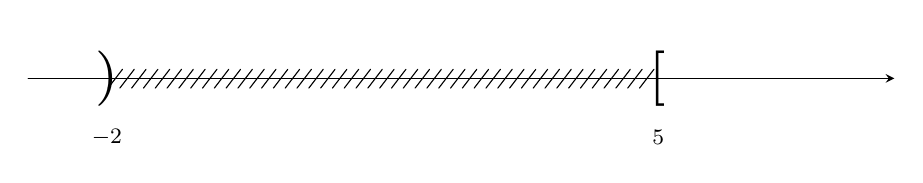
\begin{tikzpicture}[font=\footnotesize, line join=round, line cap=round, >=stealth]
\draw[-stealth](-3,0)--(8,0);
\foreach \i in{-1.9,-1.75,...,4.85}
\draw ([shift={(-125:0.15)}]\i,0)--([shift={(50:0.15)}]\i,0);
\path (-2,0)node[scale=2.5]{$)$}++(-90:0.75)node{$-2$}(5,0)node[scale=2.5]{$[$}++(-90:0.75)node{$5$};
\end{tikzpicture}
\end{center}
\choice
{\True $(-\infty;-2)\cup[5;+\infty)$}
{$(-\infty;-2)\cup(5;+\infty)$}
{$(-\infty;-2]\cup(5;+\infty)$}
{$(-\infty;-2]\cup[5;+\infty)$}
\loigiai{
Hình vẽ biểu diễn tập hợp $(-\infty;-2)\cup[5;+\infty)$.}
\end{ex}

\begin{ex}%[0D1H3-5]%[Đề chuẩn hóa số 2]%[BCTuan]
Trong một hoạt động thể thao tổ chức tại hội trại, lớp $10$A có $15$ học sinh đăng kí chơi môn đá cầu, $20$ học sinh đăng kí chơi môn cầu lông. Tìm số học sinh đăng kí chơi cả hai môn biết lớp $10$A có $40$ học sinh và có $10$ học sinh không đăng kí chơi cả hai môn đá cầu và cầu lông.
\choice
{\True $5$}
{$6$}
{$4$}
{$3$}
\loigiai{
Số học sinh của lớp $10$A biết chơi cả hai môn đá cầu và cầu lông là
\[20+15-30=5.\]
}
\end{ex}

\begin{ex}%[HK1, THPT Chuyên Hùng Vương - Phú Thọ, 2023-2024]%[Lê Quốc Hiệp, 10-11EX-HK1-2324]%[0D2N1-1]
Bất phương trình nào dưới đây là bất phương trình bậc nhất hai ẩn?
\choice
{\True $2x-y \leq 3$}
{$x^2-2y>9$}
{$xy-2x<4$}
{$\sqrt{x}-2\sqrt{y}>6$}
\loigiai
{
Bất phương trình bậc nhất hai ẩn là $2x-y \leq 3$.
}
\end{ex}

\begin{ex}%[Anh Duy, Dự án EX-10+11-M25]%[0D2H1-2]
\immini{
Phần gạch chéo trong hình vẽ sau (không kể bờ) biểu diễn miền nghiệm của bất phương trình nào trong các bất phương trình sau?
\choice
{$x-2y<3$}
{$x-2y>3$}
{\True $2x-y<3$}
{$2x-y>3$}}{
\begin{tikzpicture}[scale=.6, font=\footnotesize, line join=round, line cap=round, >=stealth]
\tikzset{every node/.style={scale=1}}
\begin{scope}[opacity=.65]
\clip (-2,-4) rectangle (4,4);
\fill[pattern=north west lines] (-3,-9)--(5,-9)--(5,7)--cycle;
\draw (3.5,4)--(-0.5,-4) node [pos=0.45, above, sloped] {$\empty$};
\end{scope}
\draw[->] (-2,0)--(4,0) node[below right]{$x$};
\draw[->] (0,-4)--(0,4) node[left]{$y$};
\draw (0,0) node[below left]{$O$};
\foreach \x in {3/2}
\draw[thin] (\x,1pt)--(\x,-1pt) node [above left] {$\dfrac{3}{2}$};
\foreach \y in {-3}
\draw[thin] (1pt,\y)--(-1pt,\y) node [left] {$\y$};
\draw[dashed,thin] (0,0)--(0,-3)--(0,-3);
\draw[dashed,thin] (3/2,0)--(3/2,0)--(0,0);
\end{tikzpicture}}
\loigiai{Ta thấy tọa độ điểm $O(0;0)$ không thỏa các bất phương trình $x-2 y>3$, $2 x-y>3$.\\
Mặt khác, nửa mặt phẳng chứa $O$, phần không bị gạch, có bờ là đường thẳng đi qua các điểm $(0;-3)$, $\left(\dfrac{3}{2};0\right)$. Đó là đường thẳng $2x-y=3$.\\
Vậy phần không bị gạch trong hình (không kể bờ) là miền nghiệm của bất phương trình $2 x-y<3$.}
\end{ex}

\begin{ex}%[De-chuan-hoa-so-1]%[Diamond]%[0D2N2-1]
Trong các hệ bất phương trình sau, hệ nào là hệ bất phương trình bậc nhất hai ẩn?
\choice
{\True $\heva{&2 x+\sqrt{3} y \geq 0 \\ &x-y<1}$}
{$\heva{&2 x+y^2 \geq 1 \\ &y+4<0}$}
{$\heva{&x^2+3 y \geq 0 \\ &x-y+4<0}$}
{$\heva{&x-3 y \geq 0 \\ &x y-y<4}$}
\loigiai{
Hệ bất phương trình bậc nhất hai ẩn là $\heva{&2 x+\sqrt{3} y \geq 0 \\ &x-y<1.}$
}
\end{ex}

\begin{ex}%[0D2H2-2]%[KNTT - Lớp 10 - Ôn tập cuối học kì 1 - Đề 03]%[Nguyễn Hữu Chung Kiên]
Điểm nào sau đây \textbf{không} thuộc miền nghiệm của hệ bất phương trình $\heva{&2x+3y-1 > 0 \\ &5x-y+4 < 0.}$
\choice
{$(-1;4)$}
{$(-2;4)$}
{\True $(0;0)$}
{$(-3;4)$}
\loigiai{Ta thấy toạ độ điểm  $O(0;0)$ \textbf{không} thoả miền nghiệm của hệ bất phương trình $\heva{&2x+3y-1 > 0 \\ &5x-y+4 < 0.}$}
\end{ex}

\begin{ex}%[HKI, Phan Bội Châu- Bình Thuận, 2023]%[Hiếu Phan]%[0H4N2-1]
Cho tam giác $ABC$ với $BC=a,\,CA=b,\,AB=c.$ Mệnh đề nào sau đây là \textbf{sai}?
\choice
{$c=\dfrac{a\sin C}{\sin A}$}
{\True $a=\dfrac{c\sin A}{\sin B}$}
{$b=\dfrac{a\sin B}{\sin A}$}
{$a=\dfrac{b\sin A}{\sin B}$}
\loigiai{
Theo định lý Sin ta có  $\dfrac{a}{\sin A}=\dfrac{c}{\sin C}\Rightarrow a=\dfrac{c\sin A}{\sin C}$ nên $a=\dfrac{c\sin A}{\sin B}$ sai.
}
\end{ex}

\begin{ex}%[24-25-Bai-Giang-K10-K11, Tran Quoc]%[0H4N2-2]
Cho hình bình hành $ABCD$ có $AB=a$, $BC=a\sqrt {3}$ và $\widehat{BAD}=120^\circ$. Diện tích của hình bình hành $ABCD$ bằng
\choice
{\True $\dfrac {3{a^2}}{2}$}
{ $3{a^2}$}
{ $\sqrt {3}{a^2}$}
{ $\dfrac {3{a^2}}{4}$}
\loigiai{
\immini{
Do $ABCD$ là hình bình hành nên ta có
\[\widehat{ABC}=180^\circ-\widehat{BAD}=180^\circ-120^\circ=60^\circ.\]
Do đó
\begin{align*}
S_{\triangle ABC}&=\dfrac{1}{2}\cdot AB\cdot BC\cdot \sin \widehat{ABC}\\
&=\dfrac{1}{2}\cdot a\cdot a\sqrt{3}\cdot \sin 60^\circ=\dfrac{3a^2}{4}.
\end{align*}
Vậy $S_{ABCD}=2S_{\triangle ABC}=\dfrac{3a^2}{2}$.}
{\begin{tikzpicture}[font=\footnotesize,line join=round, line cap=round, >=stealth,scale=0.8]
\foreach \x/\y/\pos in {0/0/A, 5/0/D} \path ($(\x,\y)$) coordinate (\pos);
\path ($(A)+(120:3)$) coordinate (B)
($(B)+(D)$) coordinate (C);
\draw (A)--(B)--(C)--(D)--(A);
\foreach \x/\pos in {A/-150, B/150, C/30, D/-30} \fill (\x) circle(1pt) node[{shift=(\pos:0.25)}]{$\x$};
\pic["$120^\circ$",draw,angle radius=7mm] {angle= D--A--B};
\end{tikzpicture}}}
\end{ex}

\begin{ex}%[0H4H2-1]%[CD-Lớp 10-Ôn tập cuối học kì 1-Đề 5]%[Hoàng Ngọc Lâm]
Biết đường tròn đi qua ba đỉnh của tam giác $A B C$ có bán kính bằng $3$ và tam giác $A B C$ có góc $\widehat{C}=60^{\circ}$. Độ dài cạnh $A B$ của tam giác $A B C$ bằng
\choice
{\True $3 \sqrt{3}$}
{$3$}
{$\sqrt{3}$}
{$\dfrac{3 \sqrt{3}}{2}$}
\loigiai{
Áp dụng định lí sin cho $\triangle A B C$, ta có \[\dfrac{A B}{\sin C}=2 R \Rightarrow A B=2 R \cdot \sin C=2 \cdot 3 \cdot \dfrac{\sqrt{3}}{2}=3 \sqrt{3}.\]
}
\end{ex}

\begin{ex}%[0H4H1-2]%[CD - Lớp 10 - Ôn tập cuối học kì 1 - Đề 6]%[Vũ Hồng Toàn]
Cho góc $a, 90^{\circ} < a < 180^{\circ}$ thỏa mãn $\sin a=\dfrac{3}{5}$. Tìm $\cos a$.
\choice
{$\dfrac{4}{5}$}
{$-\dfrac{3}{4}$}
{$-\dfrac{3}{5}$}
{\True $-\dfrac{4}{5}$}
\loigiai{
Ta có $\sin ^2a+\cos ^2a=1\Leftrightarrow \cos a=\pm \sqrt{1-\sin ^2a}=\pm \sqrt{1-\left(\dfrac{3}{5}\right)^2}=\pm \dfrac{4}{5}$.\\
Vì $90^{\circ} < a < 180^{\circ}$ nên nhận giá trị $\cos a=-\dfrac{4}{5}$.
}
\end{ex}

\begin{ex}%[Mức 2]%[BG - 10 New - 4in1,Phú Thạch]%[0H5N1-3]
Chọn khẳng định sai trong các khẳng định sau?
\choice
{ Hai véc-tơ bằng nhau thì cùng hướng}
{Hai véc-tơ bằng nhau thì có độ dài bằng nhau}
{\True Hai véc-tơ có độ dài bằng nhau thì bằng nhau}
{Hai vec-tơ đối nhau có độ dài bằng nhau}
\loigiai
{ Hai véc-tơ bằng nhau là hai véc-tơ có cùng hướng và cùng độ dài. Do đó hai véc-tơ có độ dài bằng nhau thì chưa chắc bằng nhau.}
\end{ex}

\begin{ex}%[HK1, THPT Chuyên Hùng Vương - Phú Thọ, 2023-2024]%[Lê Quốc Hiệp, 10-11EX-HK1-2324]%[0H5N2-2]
Cho hai điểm phân biệt $A$ và $B$. Gọi $I$ là trung điểm đoạn thẳng $AB$. Đẳng thức nào sau đây đúng?
\choice
{$\overrightarrow{IA}-\overrightarrow{IB}=\overrightarrow{0}$}
{$\overrightarrow{IA}+\overrightarrow{IB}=\overrightarrow{AB}$}
{$\overrightarrow{IA}-\overrightarrow{IB}=\overrightarrow{AB}$}
{\True $\overrightarrow{IA}+\overrightarrow{IB}=\overrightarrow{0}$}
\loigiai
{
Do  $I$ là trung điểm đoạn thẳng $AB$ nên $\overrightarrow{IA}+\overrightarrow{IB}=\overrightarrow{0}$.
}
\end{ex}

\begin{ex}%[0H5H2-2]%[Nguyễn Thắng,DA3-DC-NTH-T10]
Cho hình bình hành $ABCD$ và gọi I là giao điểm của hai đường chéo. Trong các khẳng định sau, khẳng định nào đúng?
\choice
{\True $\overrightarrow{IA}+\overrightarrow{DC}=\overrightarrow{IB}$}
{$\overrightarrow{AB}+\overrightarrow{AD}=\overrightarrow{BD}$}
{$\overrightarrow{IA}+\overrightarrow{BC}=\overrightarrow{IB}$}
{$\overrightarrow{AB}+\overrightarrow{IA}=\overrightarrow{BI}$}
\loigiai{
\begin{center}
\begin{tikzpicture}[scale=1, font=\footnotesize, line join=round, line cap=round, >=stealth]
\path (0,0) coordinate (A)
(-3,-2) coordinate (B)
(2,-2) coordinate (C)
($(A)+(C)-(B)$) coordinate (D)
($(A)!0.5!(C)$) coordinate (I)
;
\draw (A)--(B)--(C)--(D)--(A)--(C) (B)--(D)
;
\foreach \p/\r in {A/90,B/-90,C/-45,D/0,I/90}
\fill (\p) circle (1.2pt) node[shift={(\r:3mm)}]{$\p$};
\end{tikzpicture}
\end{center}
Vì $I$ là giao điểm của hai đường chéo nên $I$ là trung điểm của $AC$ và $BD$.\\
Suy ra $\overrightarrow{IA}=\overrightarrow{CI}$, $\overrightarrow{DI}=\overrightarrow{IB}$.\\
Khi đó $\overrightarrow{IA}+\overrightarrow{DC}=\overrightarrow{CI}+\overrightarrow{DC}=\overrightarrow{DI}=\overrightarrow{IB}$.
}
\end{ex}

\begin{ex}%[0-HK1-CD-3-DongAnh-HaNoi-2324]%[VN-MT-6, VN-22]%[0H5H3-2]
Cho tam giác $ABC$ có trọng tâm $G$, $M$ là trung điểm $BC$, mệnh đề nào sau đây đúng?
\choice
{\True $\overrightarrow{GB}+\overrightarrow{GC}=2\overrightarrow{GM}$}
{$\overrightarrow{GA}+\overrightarrow{GB}=\overrightarrow{GC}$}
{$\overrightarrow{GB}+\overrightarrow{GC}=2\overrightarrow{GA}$}
{$\overrightarrow{AB}+\overrightarrow{AC}=2\overrightarrow{AG}$}
\loigiai{
\begin{center}
\begin{tikzpicture}[line join = round,line cap = round, font = \footnotesize, scale = 1]
\path
(0:0) coordinate (B)
+(0:5) coordinate (C)
+(70:3) coordinate (A)
($(A)!.5!(B)$) coordinate (N)
($(B)!.5!(C)$) coordinate (M)
($(A)!.5!(C)$) coordinate (P)
(intersection of A--M and B--P) coordinate (G)
;
\draw
(A)--(B)--(C)--cycle
(A)--(M)
(B)--(G)--(C)
;
\foreach \x/\g in {B/180,C/0,A/90,M/-90,G/70}
\fill (\x) circle (1pt)
+(\g:3mm) node{$\x$};
\end{tikzpicture}
\end{center}
Ta có $\overrightarrow{GB}+\overrightarrow{GC}=\overrightarrow{GM}+\overrightarrow{MB}+\overrightarrow{GM}+\overrightarrow{MC}=2\overrightarrow{GM}+\overrightarrow{MB}+\overrightarrow{MC}$.\\
Vì $M$ là trung điểm của $BC$ nên ta có $\overrightarrow{MB}+\overrightarrow{MC}=\overrightarrow{0}$.\\
Vậy $\overrightarrow{GB}+\overrightarrow{GC}=2\overrightarrow{GM}$.
}
\end{ex}

\begin{ex}%[0H5N4-1]%[CD-Lớp 10-Ôn tập cuối học kì 1-Đề 5]%[Hoàng Ngọc Lâm]
Cho tam giác $A B C$ đều cạnh $a$. Tích vô hướng $\overrightarrow{A B}\cdot \overrightarrow{A C}$ có giá trị là
\choice
{\True $\overrightarrow{A B}\cdot \overrightarrow{A C}=\dfrac{a^2}{2}$}
{$\overrightarrow{A B}\cdot \overrightarrow{A C}=-\dfrac{a^2}{2}$}
{$\overrightarrow{A B}\cdot \overrightarrow{A C}=\dfrac{\sqrt{3}}{2}a^2$}
{$\overrightarrow{A B}\cdot \overrightarrow{A C}=-\dfrac{\sqrt{3}}{2}a^2$}
\loigiai{
$\overrightarrow{A B} \cdot \overrightarrow{A C}=A B \cdot A C \cdot \cos A= a\cdot a \cdot \cos 60^{\circ}=\dfrac{a^2}{2}$.
}
\end{ex}

\begin{ex}%[0H5H4-2]%[CTST-Lop 10-On-tap-cuoi-hoc-ki-1-De-6]%[Trần Hưng]
Cho hai véc tơ $\overrightarrow{a}$ và $\overrightarrow{b}$ thỏa mãn $\left|\overrightarrow{a}\right|=3$, $\left|\overrightarrow{b}\right|=2$ và $\overrightarrow{a}\cdot \overrightarrow{b}=-3$. Tính góc giữa hai véc tơ $\overrightarrow{a}$ và $\overrightarrow{b}$.
\choice
{$\left(\overrightarrow{a},\overrightarrow{b}\right)=30^{\circ}$}
{$\left(\overrightarrow{a},\overrightarrow{b}\right)=60^{\circ}$}
{$\left(\overrightarrow{a},\overrightarrow{b}\right)=45^{\circ}$}
{\True $\left(\overrightarrow{a},\overrightarrow{b}\right)=120^{\circ}$}
\loigiai{
\[
\overrightarrow{a}\cdot \overrightarrow{b}=\left|\overrightarrow{a}\right|\cdot\left|\overrightarrow{b}\right|\cdot \cos \left(\overrightarrow{a},\overrightarrow{b}\right) \Leftrightarrow \cos \left(\overrightarrow{a},\overrightarrow{b}\right)=\dfrac{\overrightarrow{a}\cdot \overrightarrow{b}}{\left|\overrightarrow{a}\right|\cdot\left|\overrightarrow{b}\right|}=\dfrac{-3}{3 \cdot 2}=\dfrac{-1}{2}.
\]
Suy ra $\left(\overrightarrow{a},\overrightarrow{b}\right)=120^{\circ}$.
}
\end{ex}

\begin{ex}%[0D8N1-1]
Trên giá sách có $10$ quyển sách Tiếng Việt khác nhau, $8$ quyển sách Tiếng Anh khác nhau và $5$ quyển sách Tiếng Pháp khác nhau. Hỏi có bao nhiêu cách chọn một quyển sách không là sách Tiếng Việt?
\choice
{$23$}
{$400$}
{\True $13$}
{$40$}
\loigiai{
Ta có thể chọn một quyển sách Tiếng Anh hoặc một quyển sách Tiếng Pháp.\\
Chọn một quyển sách Tiếng Anh: có $8$ cách.\\
Chọn một quyển sách Tiếng Pháp: có $5$ cách.\\
Có $8 + 5 = 13$ cách chọn một quyển sách không là sách Tiếng Việt.}
\end{ex}

\begin{ex}%[0D8H1-3]
Một hộp chứa $10$ quả cầu màu đỏ được đánh số từ $1$ đến $10$ và $15$ quả cầu màu xanh được đánh số từ $1$ đến $15$. Chọn ngẫu nhiên $2$ quả cầu. Hỏi có bao nhiêu cách để chọn được hai quả cầu khác màu và tổng của các số trên hai quả cầu là một số lẻ?
\choice
{$70$}
{\True $75$}
{$80$}
{$85$}
\loigiai{
Để tổng của hai số là một số lẻ thì một số là số lẻ và số còn lại là số chẵn. Mặt khác, do hai quả cầu được chọn khác nhau nên ta sẽ chọn theo cách sau đây
\begin{itemize}
\item Chọn quả đỏ số chẵn và quả xanh số lẻ.
\begin{itemize}
\item Chọn $1$ quả cầu đỏ, có $5$ cách.
\item Chọn $1$ quả cầu xanh, có $8$ cách.
\end{itemize}
Trường hợp này có $5\cdot8=40$ cách.
\item Chọn quả đỏ số lẻ và quả xanh số chẵn.
\begin{itemize}
\item Chọn $1$ quả cầu đ, có $5$ cách.
\item Chọn $1$ quả cầu xanh, có $7$ cách.
\end{itemize}
Trường hợp này có  $5\cdot 7=35$ cách.
\end{itemize}
Vậy tổng cộng có tất cả $40+35=75$ cách.
}
\end{ex}

\begin{ex}%[0D8H1-2]
Một bạn học sinh có $5$ cái quần khác nhau, $7$ cái áo khác nhau. Hỏi bạn học sinh đó có bao nhiêu cách chọn $1$ bộ quần áo?
\choice{\True $35$}
{$5$}
{$7$}
{$12$}
\loigiai{
Chọn một cái quần có $5$ cách chọn.\\
Chọn một cái áo có $7$ cách chọn. \\
Theo quy tắc nhân có $5\cdot 7=35$ cách chọn.
}
\end{ex}

\begin{ex}%[0D8N2-1]%[Dự án đề kiểm tra Toán 10 HKII NH23-24-TrungKien]%[THPT TranHungDao-TPHCM]
Với $k$ và $n$ là hai số nguyên dương tùy ý thỏa mãn $k \le n$. Mệnh đề nào dưới đây đúng?
\choice
{$\mathrm{A}_n^k=\dfrac{n!}{k!\left(n-k\right)!}$}
{$\mathrm{C}_n^k=\dfrac{\left(n-k\right)!}{n!}$}
{\True $\mathrm{A}_n^k=\dfrac{n!}{\left(n-k\right)!}$}
{$\mathrm{C}_n^k=\dfrac{n!}{\left(n-k\right)!}$}
\loigiai{
Theo công thức, ta có $\mathrm{A}_n^k=\dfrac{n!}{\left(n-k\right)!}$.
}
\end{ex}

\begin{ex}%[0D8H2-3]%[Dự án đề kiểm tra Toán 10 CHKI NH23-24- lamnguyen]%[THPT - Đồng nai]
Từ các chữ số $1,2,3,4,5$ có thể lập được bao nhiêu số tự nhiên có ba chữ số đôi một khác nhau?
\choice
{\True $60$}
{$120$}
{$3125$}
{$24$}
\loigiai{
Mỗi cách lập số tự nhiên có ba chữ số đôi một khác nhau từ một tập có $5$ chữ số khác nhau và khác $0$ là một chỉnh hợp chập $3$ của $5$ phần tử.\\
Vậy số các số lập được là $\mathrm{A}_5^3=60$ (số).
}
\end{ex}

\begin{ex}%[0D8N3-2]%[HKII-NGUYỄN THÁI BÌNH 2324]%[TheHung Nguyen]
Khai triển nhị thức $(x+3y)^4$ thu được kết quả là
\choice
{$x^4-4 x^3 y+18 x^2 y^2-36 x y^3+27 y^4$}
{\True $x^4+12 x^3 y+54 x^2 y^2+108 x y^3+81 y^4$}
{$x^4+4 x^3 y+18 x^2 y^2+36 x y^3+27 y^4$}
{$x^4-12 x^3 y+54 x^2 y^2-108 x y^3+81 y^4$}
\loigiai{
Ta có $(x+3y)^4=x^4+12x^3y+54x^2y^2+108xy^3+81 y^4$.
}
\end{ex}

\begin{ex}%[0D8H3-3]%[HKII-NGUYỄN THÁI BÌNH 2324]%[TheHung Nguyen]
Tìm hệ số của số hạng chứa $x^3$ trong khai triển $(x-2)(2x+1)^4$.
\choice
{\True $-40$}
{$-24$}
{$24$}
{$40$}
\loigiai{
Ta có
\begin{eqnarray*}
(x-2)(2x+1)^4&= &x(2x+1)^4-2(2x+1)^4\\
&= & x\sum\limits_{k=0}^4 \mathrm{C}_4^k(2x)^k-2\sum\limits_{k=0}^4 \mathrm{C}_4^k(2x)^k\\
&= & \sum\limits_{k=0}^4 \mathrm{C}_4^k2^k x^{k+1}-2\sum\limits_{k=0}^4 \mathrm{C}_4^k2^k x^k
\end{eqnarray*}
Hệ số của số hạng chứa $x^3$ trong khai triển $(x-2)(2x+1)^4$ là
\[\mathrm{C}_4^22^2-2\cdot \mathrm{C}_4^32^3=-40.\]
}
\end{ex}

\begin{ex}%[Dự án Đề GK2 PNL Cấu Trúc 2025]%[Đào-V- Thuỷ]%[0H9N1-3]
Trong mặt phẳng $Oxy$, cho điểm $A(1;-4)$, điểm $B(2;-1)$. Toạ độ véc-tơ $\vec{AB}$ là
\choice
{$\vec{AB}= (-1;-3)$}
{$\vec{AB}= (3;-5)$}
{\True $\vec{AB}= (1;3)$}
{$\vec{AB}= (1;-3)$}
\loigiai
{
Ta có $\vec{AB}= (2-1; -1+4)= (1;3)$.
}
\end{ex}

\begin{ex}%[0H9H1-3]
Cho $A(3;1)$, $B(2;5)$. Tọa độ điểm $M$ thỏa mãn $2 \overrightarrow{MA}+\overrightarrow{MB} = \overrightarrow{0}$ là
\choice
{\True $\left(\dfrac{8}{3};\dfrac{7}{3}\right)$}
{$\left(\dfrac{5}{2};\dfrac{6}{2}\right)$}
{$\left(-\dfrac{5}{2};-\dfrac{6}{2}\right)$}
{$\left(-\dfrac{8}{3};-\dfrac{7}{3}\right)$}
\loigiai{Gọi tọa độ điểm $M$ cần tìm là $M(x;y)$. Khi đó $\overrightarrow{MA}=(3-x;1-y)$, $\overrightarrow{MB}=(2-x;5-y)$. \\
Ta có
\[2\overrightarrow{MA}+\overrightarrow{MB} = \overrightarrow{0} \Leftrightarrow \heva{&2(3-x)+2-x=0 \\ &2(1-y)+5-y=0} \Leftrightarrow \heva{&x=\dfrac{8}{3} \\ &y=\dfrac{7}{3}.}\]
Vậy tọa độ điểm $M$ cần tìm là $M\left(\dfrac{8}{3};\dfrac{7}{3}\right)$.}
\end{ex}

\begin{ex}%[0H9H1-3]
Cho $A(3;1)$, $B(2;5)$. Tọa độ điểm $M$ thỏa mãn $2 \overrightarrow{MA}+\overrightarrow{MB} = \overrightarrow{0}$ là
\choice
{\True $\left(\dfrac{8}{3};\dfrac{7}{3}\right)$}
{$\left(\dfrac{5}{2};\dfrac{6}{2}\right)$}
{$\left(-\dfrac{5}{2};-\dfrac{6}{2}\right)$}
{$\left(-\dfrac{8}{3};-\dfrac{7}{3}\right)$}
\loigiai{Gọi tọa độ điểm $M$ cần tìm là $M(x;y)$. Khi đó $\overrightarrow{MA}=(3-x;1-y)$, $\overrightarrow{MB}=(2-x;5-y)$. \\
Ta có
\[2\overrightarrow{MA}+\overrightarrow{MB} = \overrightarrow{0} \Leftrightarrow \heva{&2(3-x)+2-x=0 \\ &2(1-y)+5-y=0} \Leftrightarrow \heva{&x=\dfrac{8}{3} \\ &y=\dfrac{7}{3}.}\]
Vậy tọa độ điểm $M$ cần tìm là $M\left(\dfrac{8}{3};\dfrac{7}{3}\right)$.}
\end{ex}

\begin{ex}%[0H9N2-1]
Cho $\vv{u}=(-2;2)$ và $\vv{v}=(4;-2)$. Tích vô hướng của $\vv{u}$ và $\vv{v}$ là
\choice
{$10$}
{$2$}
{$-8$}
{\True $-12$}
\loigiai{
Ta có $\vv{u}\cdot\vv{v}=-2\cdot 4+2\cdot (-2)=-12$.
}
\end{ex}

\begin{ex}%[Dự án EX-10-11-Chuẩn hóa]%[Hoàng Thanh Phương]%[0H9H2-2]
Trong mặt phẳng với hệ trục tọa độ $Oxy$, cho tam giác $ABC$ có $A(1;2), B(0;4), C(3;1)$. Khi đó $\cos (\overrightarrow{AB}, \overrightarrow{AC})$ bằng
\choice{\True $-\dfrac{4}{5}$}{$\dfrac{1}{2}$}{$\dfrac{4}{5}$}{$0$}
\loigiai{
Ta có $\overrightarrow{AB}=(-1;2)$, $\overrightarrow{AC}=(2;-1)$. Vậy
\[\cos (\overrightarrow{AB}, \overrightarrow{AC})=\dfrac{(-1)\cdot 2+2\cdot (-1)}{\sqrt{(-1)^2+2^2}\cdot \sqrt{2^2+(-1)^2}}=-\dfrac{4}{5}.\]
}
\end{ex}

\begin{ex}%[0H9N2-2]%[KNTT - Lớp 10 - Ôn tập cuối học kì 1 - Đề 5]%[Phạm Hải Dương]
Cho $\overrightarrow{a} = (1; -2)$, $\overrightarrow{b} = (-2; -6)$. Khi đó góc giữa chúng là
\choice
{\True $45^\circ$}
{$135^\circ$}
{$60^\circ$}
{$30^\circ$}
\loigiai{
Ta có $\cos(\overrightarrow{a}, \overrightarrow{b}) = \dfrac{1 \cdot (-2) + (-2) \cdot (-6)}{\sqrt{1^2 + (-2)^2} \cdot \sqrt{(-2)^2 + (-6)^2}} = \dfrac{\sqrt{2}}{2} \Rightarrow (\overrightarrow{a}, \overrightarrow{b}) = 45^\circ$
}
\end{ex}
\Closesolutionfile{ans}

\section{Trả lời các câu hỏi sau, trong mỗi ý a), b), c), d), \ldots ở mỗi câu, thí sinh chọn đúng hoặc sai.}
\Opensolutionfile{ans}[ans/ansDe2-TN2]
\begin{ex}%[0-HK1-KN-1-PhanDinhPhung-HaNoi-2324]%[VN-MT-6, VM019]%[0H5V3-5]
Cho tam giác $ABC$ có $M$ là trung điểm $BC$ và $G$ là trọng tâm. Lấy các điểm $E$, $F$ thỏa mãn $3\overrightarrow{EA}+2\overrightarrow{EC}=\overrightarrow{0}$ và $\overrightarrow{FA}=2\overrightarrow{FB}$.
\choiceTF
{\True $B$ là trung điểm đoạn thẳng $AF$}
{\True $\overrightarrow{FG}=2\overrightarrow{AM}-2\overrightarrow{AB}$}
{$\overrightarrow{FE}=\dfrac{2}{5}\overrightarrow{AC}+2\overrightarrow{AB}$}
{\True $\overrightarrow{FG}=\dfrac{5}{6}\overrightarrow{FE}$}
\loigiai{
\begin{center}
\begin{tikzpicture}[font=\footnotesize,line join=round, line cap=round, >=stealth,scale=1]
\path
(0,0)coordinate(B)++(0:5)coordinate(C)++(140:5)coordinate(A)
($(B)!.5!(C)$)coordinate(M)
($(A)!2!(B)$)coordinate(F)
($(A)!2/3!(M)$)coordinate(G)
(intersection of A--C and F--G)coordinate(E)
;
\draw (A)--(B)--(C)--cycle
(A)--(M) (B)--(F)--(E)
;
\foreach \x/\pos in {B/180,A/90,C/0,M/-90,E/45,G/-30,F/180} \fill (\x) circle(1pt) node[{shift=(\pos:0.25)}]{$\x$};
\end{tikzpicture}
\end{center}
\begin{itemchoice}
\itemch {\bf Đúng}.\\
Ta có $\overrightarrow{FA}=2\overrightarrow{FB}$ nên $B$ là trung điểm đoạn thẳng $AF$.
\itemch {\bf Đúng}.\\
Do $G$ là trọng tâm của $\triangle ABC$ nên $\overrightarrow{AG}=\dfrac{2}{3}\overrightarrow{AM}$.\\
Khi đó, $\overrightarrow{FG}=\overrightarrow{AG}-\overrightarrow{AF}=\dfrac{2}{3}\overrightarrow{AM}-2\overrightarrow{AB}$.
\itemch {\bf Sai}.\\
Ta có $3\overrightarrow{EA}+2\overrightarrow{EC}=\overrightarrow{0}\Leftrightarrow 3\overrightarrow{EA}+2\overrightarrow{EA}+2\overrightarrow{AC}=\overrightarrow{0}\Leftrightarrow\overrightarrow{AE}=\dfrac{2}{5}\overrightarrow{AC}$.\\
Khi đó, $\overrightarrow{FE}=\overrightarrow{AE}-\overrightarrow{AF}=\dfrac{2}{5}\overrightarrow{AC}-2\overrightarrow{AB}$.
\itemch {\bf Đúng}.\\
Ta có
\allowdisplaybreaks
\begin{eqnarray*}
\overrightarrow{FG}&=&\overrightarrow{AG}-\overrightarrow{AF}\\
&=&\dfrac{2}{3}\overrightarrow{AM}-2\overrightarrow{AB}\\
&=&\dfrac{2}{3}\cdot\dfrac{1}{2}\left(\overrightarrow{AB}+\overrightarrow{AC}\right)-2\overrightarrow{AB}\\
&=&-\dfrac{5}{3}\overrightarrow{AB}+\dfrac{1}{3}\overrightarrow{AC}\\
&=&\dfrac{5}{6}\left(\dfrac{2}{5}\overrightarrow{AC}-2\overrightarrow{AB}\right)\\
&=&\dfrac{5}{6}\overrightarrow{FE}.
\end{eqnarray*}
\end{itemchoice}
}
\end{ex}

\begin{ex}%[0-HK1-CT-4-THTHDHSG-HCM-2324]%[VN-MT-6, VM026]%[0H5V4-4]
Cho hình vuông $ABCD$ cạnh $a$ có $M$ là trung điểm của đoạn thẳng $AB$ và $N$ là điểm thuộc đoạn thẳng $AC$ sao cho $NA=3NC$.
\choiceTF
{\True $\overrightarrow{AB}\cdot\overrightarrow{AC}=a^2$}
{$\overrightarrow{DN}=\dfrac{3}{4}\overrightarrow {AB}+\dfrac{1}{4}\overrightarrow {AD}$}
{\True $\overrightarrow{MN}=\dfrac{1}{4}\overrightarrow{AB}+\dfrac{3}{4}\overrightarrow {AD}$}
{\True $DN$ vuông góc với $MN$}
\loigiai{
\begin{center}
\begin{tikzpicture}[scale=1, font=\footnotesize, line join=round, line cap=round, >=stealth]
\def\a{4} %cạnh
\path (0:0) coordinate (B)
++(0:\a) coordinate (C)
++(90:\a) coordinate (D)
++(180:\a) coordinate (A);
\path ($(A)!0.5!(B)$) coordinate (M);
\path ($(A)!3/4!(C)$) coordinate (N);
\draw (A)--(B)--(C)--(D)--cycle;
\draw (A)--(C) (D)--(N)--(M);
\foreach \x/ \goc in {A/135,B/-135,C/-45,D/45, M/180, N/0}
\fill (\x) circle (1pt)
($(\x)+(\goc:3mm)$) node {$\x$};
\end{tikzpicture}
\end{center}
\begin{itemchoice}
\itemch {\bf Đúng}.\\
Ta có $\overrightarrow{AB}\cdot\overrightarrow{AC}=\left|\overrightarrow{AB}\right|\cdot\left|\overrightarrow{AC}\right|\cdot\cos\left(\overrightarrow {AB},\overrightarrow {AC}\right)=AB\cdot AC\cdot\cos\widehat{BAC}=a\cdot a\sqrt{2}\cdot \dfrac{\sqrt{2}}{2}=a^2$.
\itemch {\bf Sai}.\\
Phân tích vectơ $\overrightarrow{DN}$ theo hai vectơ $\overrightarrow{AB}$ và $\overrightarrow{AD}$.\\
Ta có
\begin{eqnarray*}
&\overrightarrow{DN} & =\overrightarrow {AN}-\overrightarrow {AD}=\dfrac{3}{4}\overrightarrow {AC}-\overrightarrow{AD} =\dfrac{3}{4}\left(\overrightarrow {AB}+\overrightarrow {AD}\right)-\overrightarrow{AD}=\dfrac{3}{4}\overrightarrow {AB}-\dfrac{1}{4}\overrightarrow {AD}.
\end{eqnarray*}
\itemch {\bf Đúng}.\\
Ta có $\overrightarrow{AN}=\dfrac{3}{4}\overrightarrow{AC}$, $\overrightarrow{AM}=\dfrac{1}{2}\overrightarrow{AB}$.\\
$\overrightarrow{MN}=\overrightarrow{AN}-\overrightarrow{AM}=\dfrac{3}{4}\left(\overrightarrow{AB}+\overrightarrow{AD}\right)-\dfrac{1}{2}\overrightarrow {AB}=\dfrac{1}{4}\overrightarrow{AB}+\dfrac{3}{4}\overrightarrow {AD}$.
\itemch {\bf Đúng}.
\begin{eqnarray*}
&\overrightarrow{DN}\cdot\overrightarrow{MN}& =\left(\dfrac{3}{4}\overrightarrow {AB}-\dfrac{1}{4}\overrightarrow{AD}\right)\left(\dfrac{1}{4}\overrightarrow {AB}+\dfrac{3}{4}\overrightarrow{AD}\right)\\
&& =\dfrac{3}{4}\cdot \dfrac{1}{4} \overrightarrow {AB} \cdot \overrightarrow {AB} + \dfrac{3}{4}\cdot \dfrac{3}{4}\cdot \overrightarrow {AB} \cdot \overrightarrow {AD} - \dfrac{1}{4} \cdot \dfrac{1}{4} \cdot \overrightarrow {AB} \cdot \overrightarrow {AD} - \dfrac{1}{4} \cdot \dfrac{3}{4} \cdot \overrightarrow {AD} \cdot \overrightarrow {AD}\\
&&=\dfrac{3}{16}AB^2+0-0-\dfrac{3}{16}AD^2=\dfrac{3}{16}AB^2-\dfrac{3}{16}AD^2\\
&&=0.
\end{eqnarray*}
Vậy $DN$ vuông góc với $MN$.
\end{itemchoice}
}
\end{ex}

\begin{ex}%[0-HK1-KN-1-PhanDinhPhung-HaNoi-2324]%[VN-MT-6, VM019]%[0H9V2-4]
Trong mặt phẳng tọa độ $Oxy$, cho tứ giác $ABCD$ với $A(-1;4)$, $B(4;3)$, $C(8;-3)$, $D(-2;-1)$.
\choiceTF
{\True Độ dài cạnh $AB=\sqrt{26}$}
{\True $AB+AD=CD$}
{Điểm $M$ thỏa mãn $2\overrightarrow{MA}-2\overrightarrow{MB}+4\overrightarrow{MC}=\overrightarrow{MD}$ có tọa độ $(8;3)$}
{\True $ABCD$ là hình thang vuông}
\loigiai{
\begin{itemchoice}
\itemch {\bf Đúng}.\\
Ta có $AB=\sqrt{(4+1)^2+(3-4)^2}=\sqrt{26}$.
\itemch {\bf Đúng}.\\
$AD=\sqrt{(-2+1)^2+(-1-4)^2}=\sqrt{26}$ và $CD=\sqrt{(-2-8)^2+(-1+3)^2}=2\sqrt{26}$.\\
Do đó, $AB+AD=CD=2\sqrt{26}$.
\itemch {\bf Sai}.\\
Đặt $M(x;y)$. Ta có
\begin{multicols}{2}
\begin{itemize}
\item $\overrightarrow{MA}=(-1-x;4-y)$;
\item $\overrightarrow{MB}=(4-x;3-y)$;
\item $\overrightarrow{MC}=(8-x;-3-y)$;
\item $\overrightarrow{MD}=(-2-x;-1-y)$.
\end{itemize}
\end{multicols}
Từ hệ thức $2\overrightarrow{MA}-2\overrightarrow{MB}+4\overrightarrow{MC}=\overrightarrow{MD}$, ta có
\[\heva{&2(-1-x)-2(4-x)+4(8-x)=-2-x\\&2(4-y)-2(3-y)+4(-3-y)=-1-y}\Leftrightarrow\heva{&-3x=-24\\&-3y=9}\Leftrightarrow\heva{&x=8\\&y=-3.}\]
Vậy $M(8;-3)$.
\itemch {\bf Đúng}.\\
Ta có $\overrightarrow{AB}=(5;-1)$; $\overrightarrow{AD}=(-1;-5)$; $\overrightarrow{CD}=(-10;2)$.\\
Khi đó, $\heva{&\overrightarrow{AB}\cdot\overrightarrow{AD}=5\cdot (-1)-1\cdot (-5)=0\\&\overrightarrow{CD}\cdot\overrightarrow{AD}=-10\cdot (-1)+2\cdot (-5)=0}\Rightarrow\heva{&AB\perp AD\\&CD\perp AD.}$\\
Suy ra, $AB\parallel CD$.\\
Khi đó, $ABCD$ là hình thang vuông.
\end{itemchoice}
}
\end{ex}
\Closesolutionfile{ans}
